\begin{frame}{Græsbræmmer som fodpose}

\small

\begin{columns}[T]

\begin{column}{0.58\textwidth}

\textbf{Regler for græsbræmmer som fodpose:}

\begin{itemize}[]
\item Fodpose langs søer, vandløb, kystlinjer, vådområder, levende hegn, skovbryn, markskel og lign.
\item Består primært af græsser og urtevegetation
\item Min. 2 m bred
\item Min. 50\% soleksponeret
\item Må ikke gødskes eller sprøjtes
\end{itemize}

\vspace{0.4em}

\textbf{Gavner arter:}

\footnotesize
Agerhøne, fasan, hare, rådyr, sanglærke, vibe, gul vipstjert, rødrygget tornskade, 
gulspurv, markpiber, vilde bier, humlebier, dagsommerfugle, rovbiller, græshopper, 
overvintrende insekter, markmus, pindsvin, lækat, flagermus, musvåge, tårnfalk

\end{column}

\begin{column}{0.40\textwidth}
\centering
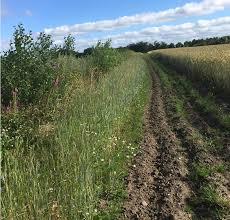
\includegraphics[width=\textwidth]{Billeder/Vildtforvaltning/biotopplantiltag/græsbræmme.jpeg}
\end{column}

\end{columns}

\end{frame}